\documentclass[10pt,a4paper]{article}

%\usepackage{lipsum}
%\usepackage{here}
%\usepackage{qtree}
%\usepackage{amstext}
%\usepackage{multirow}
%\usepackage{subfigure}
%\usepackage{algorithm}
%\usepackage{algorithmic}
%\usepackage{listings}
%\usepackage{xcolor}

\usepackage{verbatim}
\usepackage{url}
\usepackage{amsmath}
\usepackage[UKenglish]{isodate}
\usepackage{graphicx}
\usepackage{multicol}
\usepackage{caption}
\usepackage{multicol}
\usepackage[margin=0.67in]{geometry} %margins usually 0.67

\begin{document}

\title{Automation of Crystal Orientation}
\author{Aidan  Boxall}
\maketitle

\begin{abstract}
Beamline I16 at Diamond light Source carries out experiments looking at subtle magnetic properties of crystals using x-ray diffraction. Due to the small
number of crystals handled at I16 compared to other beam lines they did not have an automated crystal orientation facility. The purpose of this project was
to produce python code that could provide an orientation matrix for a crystal of arbitrary orientation but known crystal structure.
\end{abstract}

\begin{multicols}{2}
\section*{Introduction}

\section*{Choosing Bragg Reflections}
The first aim of the project was to write a python script that could choose appropriate Bragg reflections to use for crystal orientation. This was achieved 
by considering many factors and giving them appropriate weightings.
\subsubsection*{Rotational Symmetry}
The list of reflections to choose from was reduced by a filter which removes the Bragg reflections which have a higher order of rotational symmetry than the
 crystal. This was necessary because if the rotational symmetry of the Bragg reflections is higher than that of the crystal it is not possible to find 
 the correct orientation matrix all of the time. In this situation there will be a set of at least two possible non-equivalent orientation matrices and only
one will be the true orientation matrix of the crystal. 
\subsubsection*{Nearby Reflections}
It is important to consider how many reflection are nearby to the group under consideration. If the crystal has other reflection which occur at nearby
 values of two theta then it is possible they will appear on the detector whilst scanning for the desired reflections. This could be problematic if one
 reflection is so close to another that either they cannot be distinguished or they could be mistaken for one another.
\subsubsection*{Ideal Reflection Angle}
Ideally the two theta angled needs to be around 45 degrees. If the angle is too low shadowing can become a problem %CHECK was that right?
and if its too large then chi step need to be very small. %CHECK was that right?
\subsubsection*{Number of Reflections}
After applying the filter to remove groups of equivalent reflections that have a higher rotational symmetry than the crystal it is desirable to have as many 
reflections as possible in the chosen equivalent reflection group. The more reflections possible the more there are likely to be picked up by the detector. Therefore making more data available to use to find an accurate orientation matrix.
\subsubsection*{Intensity}
Obviously reflections with a higher intensity are more desirable choices are they are easier to detect. 

\section*{Finding the Peaks}
Once the reflections had been scanned it was necessary to find the reflection peaks within the data. This was done using the following method. Normally when a scan is carried out a region of interest (ROI) is defined. This is the region of the scan image where the peaks are expected. The pixel value sums of the ROI for each are stored in a data file for the scan. If the ROI was not defined or defined incorrectly at the time the scan was taken the code produced allows for this by containing methods to define a ROI and find the pixel sums from the image data directly. This is not desirable though as it is time consuming to run. Once the ROI sums have been found the average and standard deviation of these value are calculated. This allows a minimum value for a ROI of a particular image to be considered high enough to contain a peak. This is initially considered to be the mean value plus five standard deviations. The required number of standard deviations is reduced until a desired number of peaks are found or the number reaches two. It was decided pixel counts below the mean plus two standard deviations are not significant enough to be considered peaks.

To ensure that areas around the top of peaks were not counted as peaks the following method was used. The code searches for the ROIs with the highest pixel counts. Then it looks at the neighbouring images in the kphi and chi directions. It continues to look at neighbouring images until it finds images that have ROI counts below the current minimum. It then removes all the images within this rectangular area in chi-kphi space from mask array. The mask array is an array the same size and shape as the ROI sums array but simply records which images have already been used and should no longer be counted as peaks. After all the brightest ROIs have either been listed as having peaks or have been masked the next brightest set of ROIs is considered. This process is repeated unit there are no longer any points left unmasked above the minimum peak height or the desired number of peaks is found. Then as mentioned above if the desired number of peaks has not been found the minimum peak height is reduced and the entire process is repeated.  

Once a list of images containing peaks had been found the coordinates of the peaks within the images was found by assuming the peaks were the brightest pixel in the ROI.

The peaks found in the image data were converted to momentum transfer vectors in the lab Cartesian frame using code developed by another Diamond employee.

\section*{Finding the Orientation Matrix}
Finding the orientation matrix was the most challenging and arguably the most important part of the project. Early in the planning it was realised an orientation matrix could be calculated by comparing two found momentum transfer vectors in the lab Cartesian frame to two theoretical momentum transfer vectors in the crystal Cartesian frame and finding the rotations required to transform one set to the other. The set of theoretical momentum transfer vectors consists of the entire set of vectors in the crystals reciprocal space %CHECK is it actually all of them? Isn't reciprocal space infinite? Is it a unit cell of reciprocal space?
whereas the found vectors will be typically two to four vectors in lab Cartesian space. To find the rotation that transforms one to the other it is required to find which vectors in the crystal frame correspond to the vectors in the lab frame. This requires a number of comparisons to ensure a valid set of vectors is chosen. Firstly the vectors moduli are compared to ensure they match. The vectors moduli physically corresponds to the two theta angle so must be the same for the same reflection. The angle between the vectors must also match. The angle between the vectors can be found by taking the dot product. By examining the moduli and the angle between the first pair of found vectors it is possible to find a matching pair in crystal Cartesian space. However, this is not necessarily sufficient to be sure that the correct pair has been found. This is only sufficient if the pair of vectors lie on a plane of symmetry in crystal Cartesian space. Otherwise there is an asymmetry about the chosen pair of vectors and without more information it is impossible to tell which way around the crystal is orientated. %This really needs a figure to illustrate this.
To find which way the crystal is in fact orientated a third vector needs to be considered. If the third vector is not coplanar with the first then it is possible to find which side of the first two it lies on by taking the dot product of the third vector with the cross product of the first two. If the three vectors are coplanar it is possible to match the third vector by the angles between them and moduli alone unless the first two vectors are anti-parallel. If there first two vectors are anti-parallel then they are assumed to be on an plane of symmetry in reciprocal space. Apart from coplanar vectors like this anti-parallel vectors cannot be used as the first two found vectors.

Once the first two vectors have been matched to targets the rotations need to be found. The first rotation is used to rotate the first found vector onto the first target. It can be found by choosing an axis of rotation to be the cross product of the found and target vectors and the angle of rotation to be the angle between the vectors as shown in Figure \ref{rotation1}.
\begin{center}
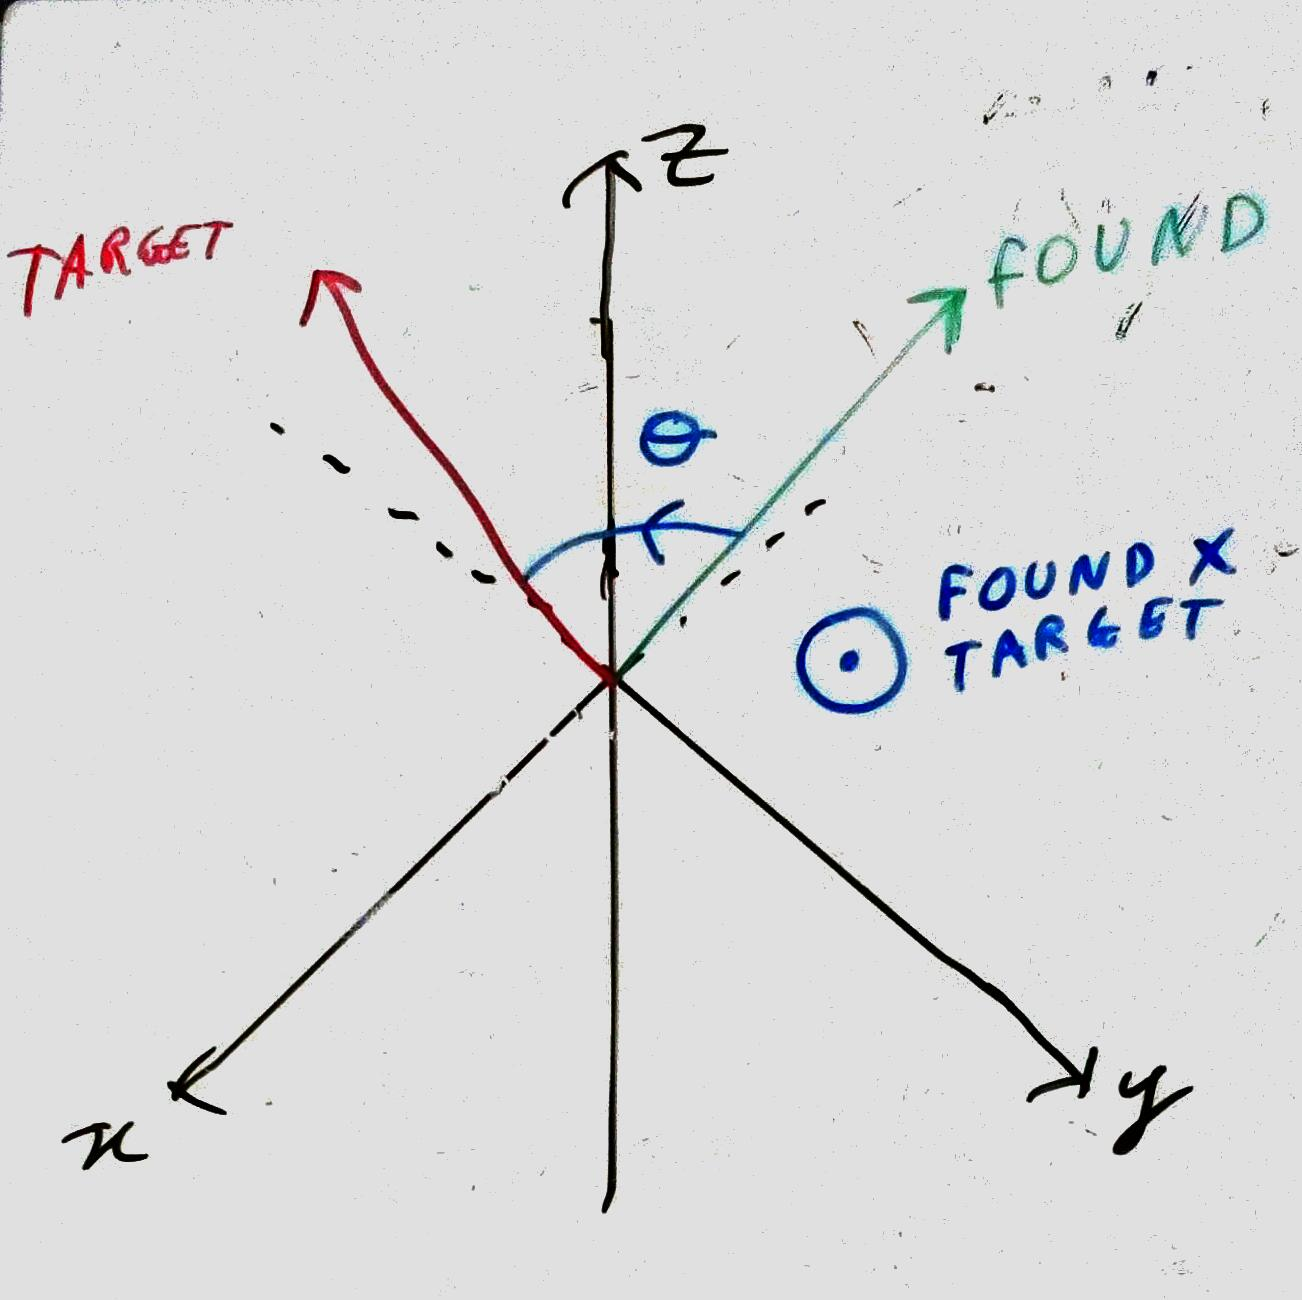
\includegraphics [width=5 cm]{rotation1.jpg}
\captionof{figure}{The first rotation.}
\label{rotation1}
\end{center}
This leaves the only possible rotation as one about the first target vector. The angle of this rotation is the angle between the components of the second found vector and the second target vector which are perpendicular to the first vector as shown in Figure \ref{rotation2}.
\begin{center}
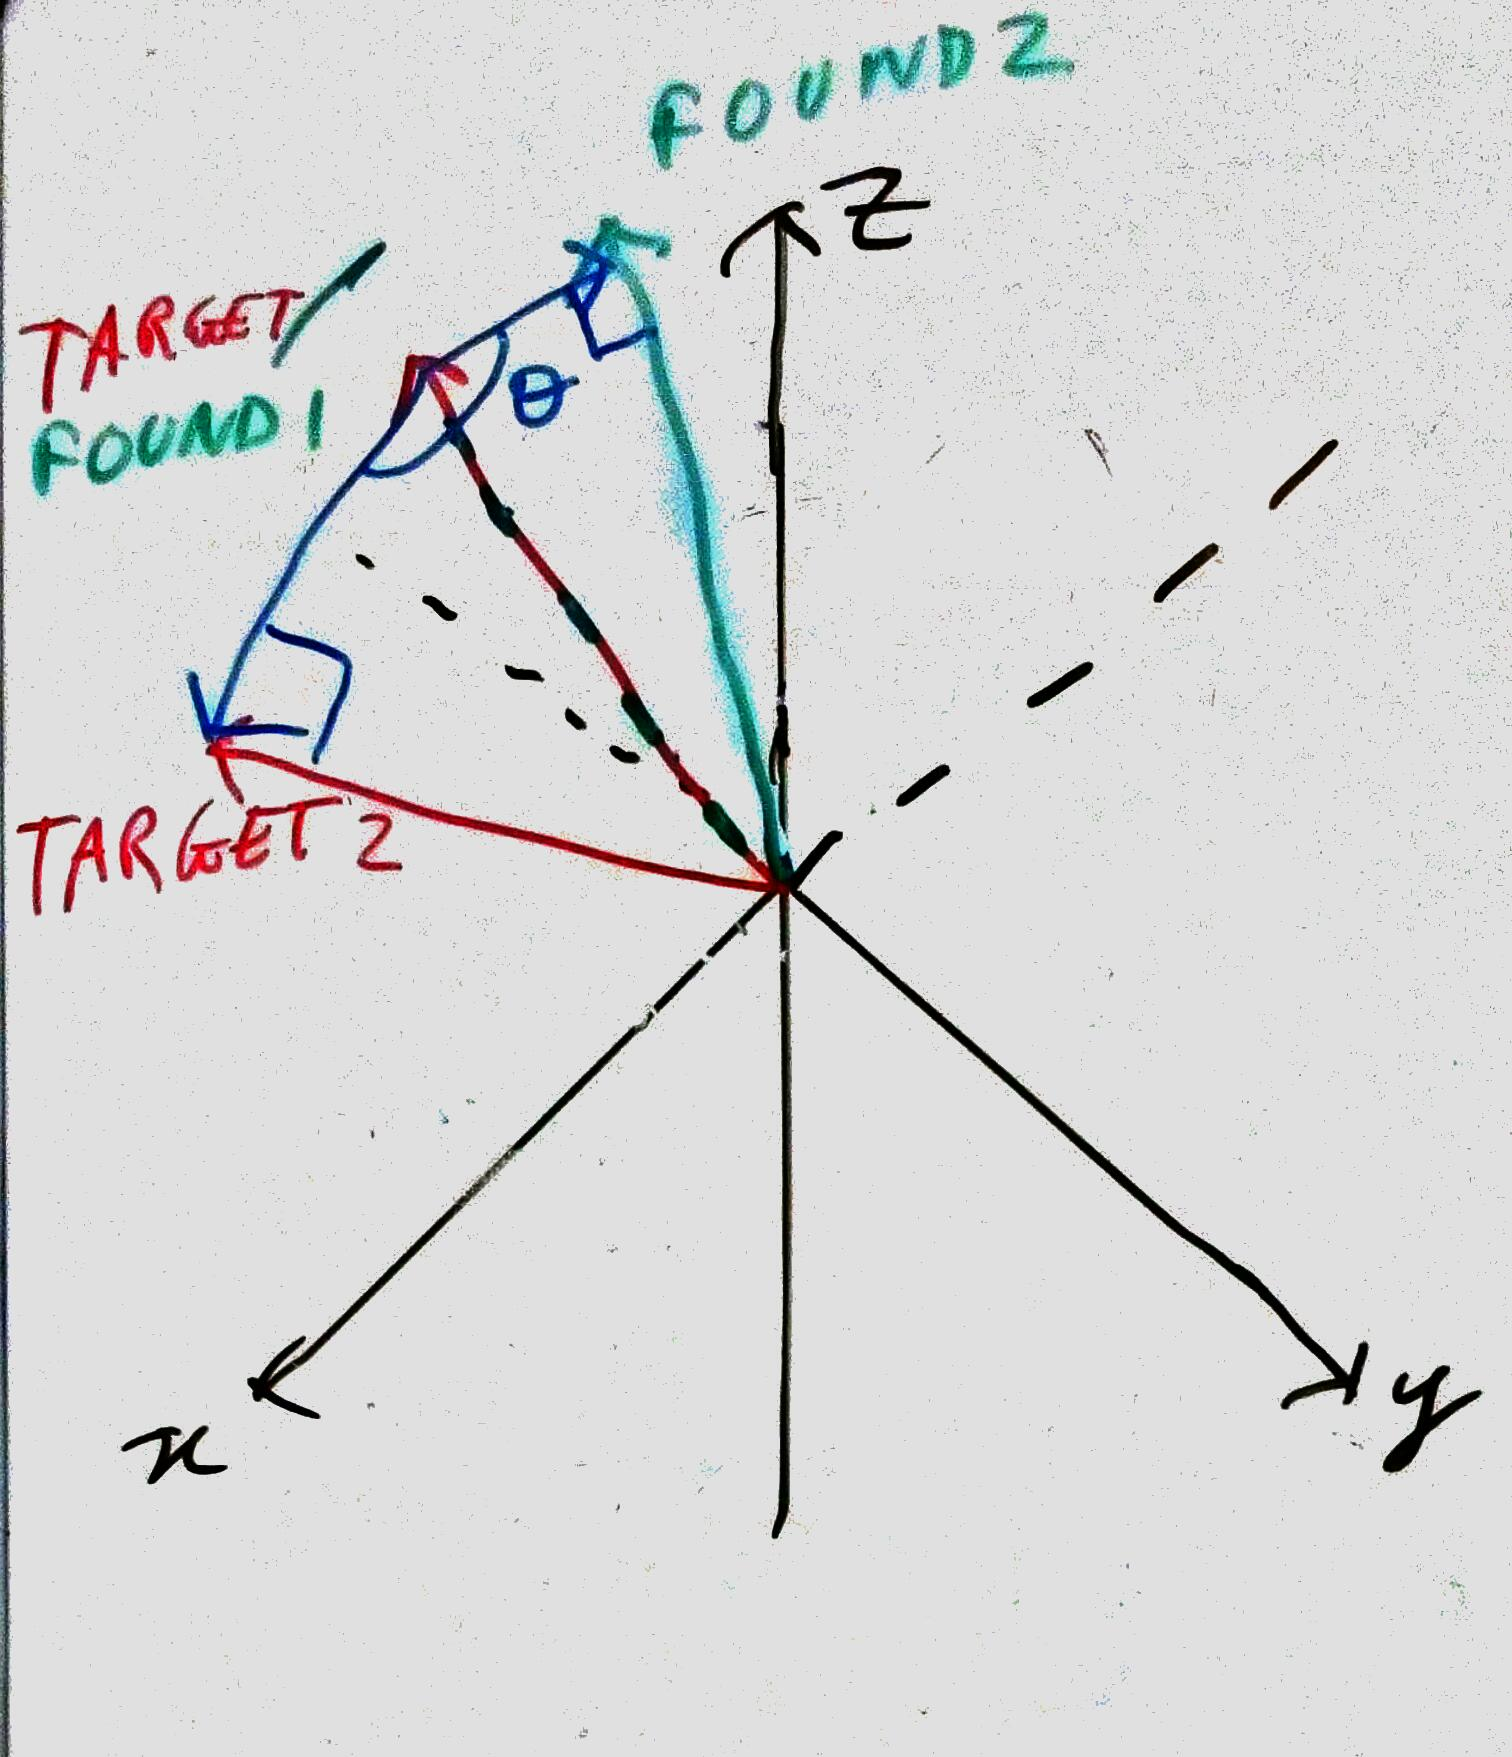
\includegraphics [width=5 cm]{rotation2.jpg}
\captionof{figure}{The second rotation.}
\label{rotation2}
\end{center}





\end{multicols}



\bibliographystyle{unsrt}
\bibliography{Bibliography}

\section*{Appendix}

\end{document}
